\section{Numerical solution}

\paragraph{Method}
To determine the stability of the upper fixed point, a fourth-order Runge-Kutta method was employed to evolve a trajectory with the initial condition $\theta_0 \simeq 0$. After a specified amount of dimensionless time had elapsed, the fixed point was defined as numerically stable if the trajectory remained within a prescribed tolerance of the fixed point $\theta = 0$. 

This process was repeated for a range of $(a, \sigma)$ values, and te results were plotted alongside the multiscale method prediction. For simplicity, the value of $\mu$ was assumed constant throughout the simulation.

\paragraph{Parameter range}
The value of $\theta_0$ must be sufficiently close to the fixed point to lie within its attraction basin, yet sufficiently far to allow feasible numerical analysis. The value chosen was $\theta_0 = 10^{-7}$, and the angular velocity $\omega_0$ was assumed to be 0.

As the multiscale method requires $\mu$ to be of order $\epsilon$, a value of $\mu = 0.1$ was chosen and held constant throughout the simulations.

The parameter $a$, which must be of order $\epsilon \simeq 0.1$, was varied within the range $0$ -- $0.3$, while $\sigma$, of order $\epsilon^2 \simeq 0.01$, was varied within the range $10^{-5}$ -- $0.02$. In this range, 30 equally spaced values were chosen for both $a$ and $\sigma$. This resolution was sufficient to capture the required behaviour while maintaining manageable computational run-times.

Table \ref{tab:params} summarizes the simulation parameters.

\begin{table}[h]
    \centering
    \begin{tabular}{|c|c|} \hline 
        $\theta_0$ & $10^{-7}$ \\ \hline 
        $\omega_0$ & 0 \\ \hline 
         $\mu$&  0.1\\ \hline
         $a$&  $0$ -- $0.3$\\ \hline
         $\sigma$&  $10^{-5}$ -- $0.02$\\ \hline
    \end{tabular}
    \caption{Parameter ranges.}
    \label{tab:params}
\end{table}


\subsection{Time step size}

The time step was selected to be sufficiently small to resolve the system's fast dynamics. Given that $\mu = \flatfrac{c}{\omega} = 0.1$, it follows that $\omega \sim \flatfrac{1}{\mu} = 10$, so the period of the pivot oscillations is of order $\flatfrac{2 \pi}{\omega} \sim 0.6$. To ensure accuracy, the time step was set approximately one order of magnitude smaller than this period, resulting in a time step of $\SI{1e-2}{}$.

To observe the fixed point's behaviour over a sufficiently large dimensionless time, the simulation was executed for $10\,000$, corresponding to a final dimensionless time of $t = 100$.


\subsection{Tolerance setting}
The tolerance for determining the stability of the fixed point was chosen based on a physical constraint: when $a = 0$ (i.e., $b = 0$), the Kapitza pendulum reduces to a regular pendulum with a stationary pivot. In this case, the upper fixed point is always unstable.

To ensure this condition was satisfied, a simple algorithm was devised to determine a suitable tolerance. The relevant implementation can be found in the code listing starting at line 38 (Listing \ref{lst:plot}).

The tolerance used was $\SI{1.01e-7}{}$.

\subsection{Comparison with multiscale method} \label{sec:com_anal_sol}

\begin{figure}[h]
    \centering
    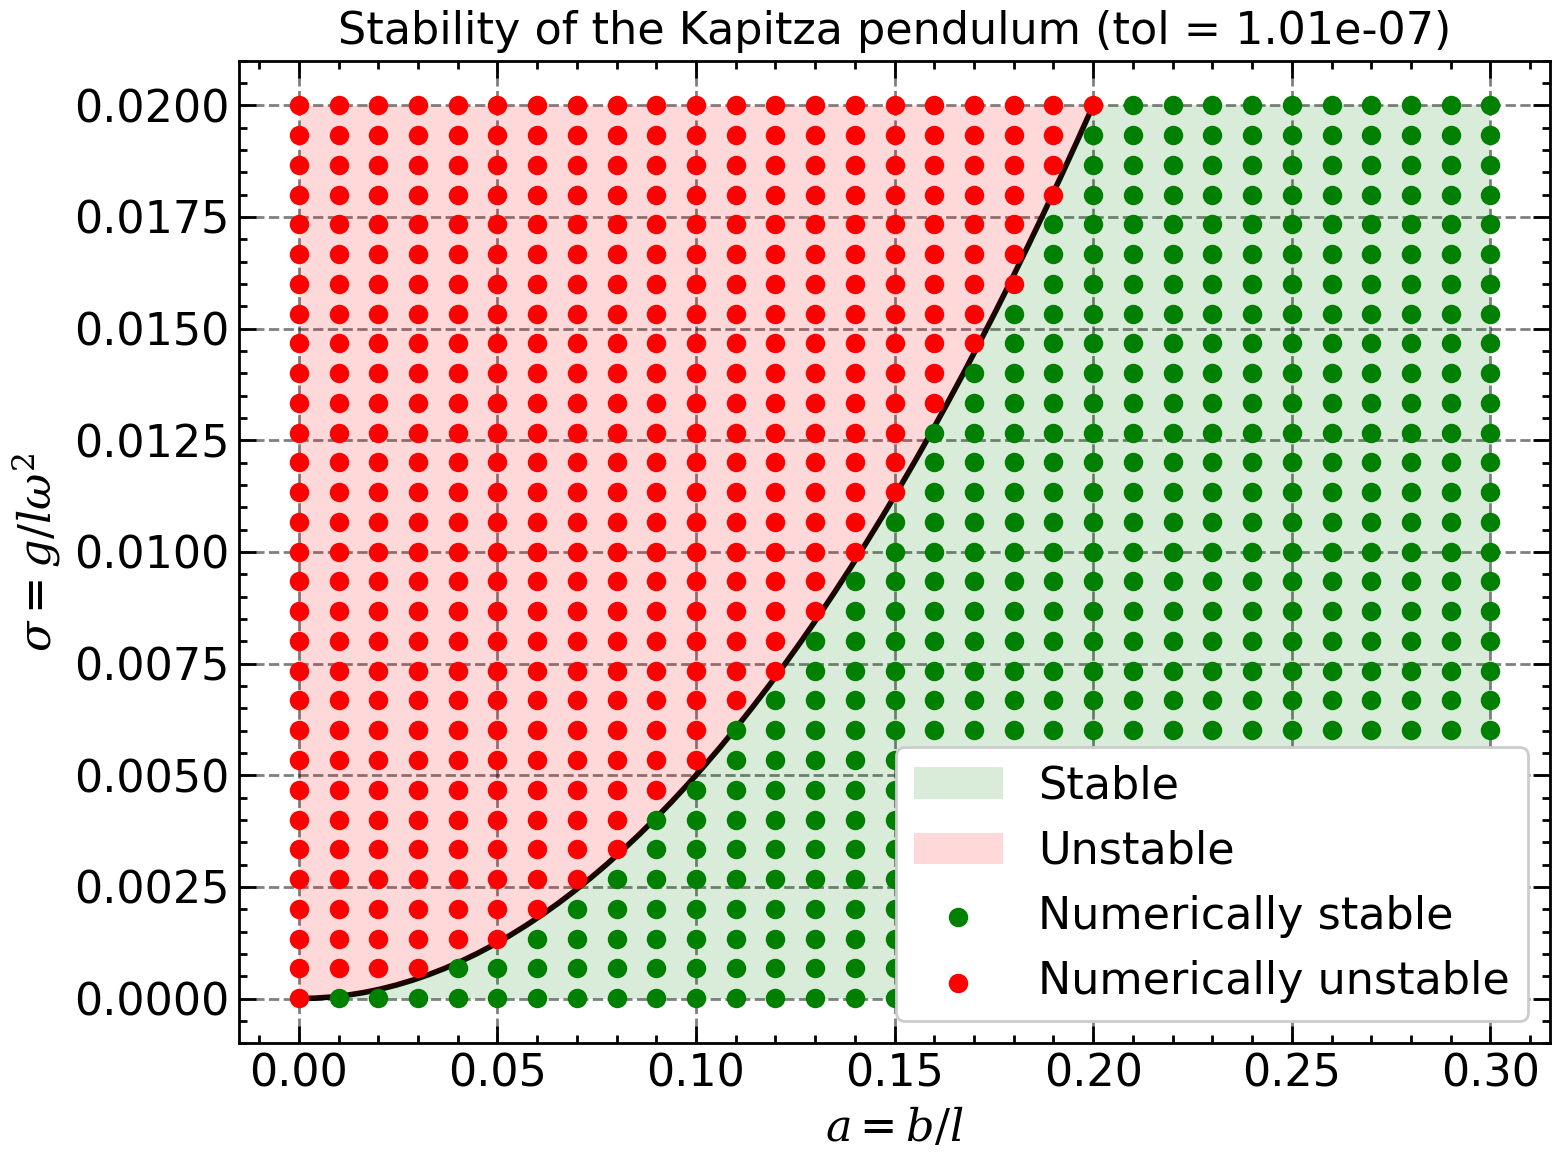
\includegraphics[width=0.75\linewidth]{Images/stability_1.01e-07.png}
    \caption{Stability of the upper fixed point.}
    \label{fig:stability}
\end{figure}

The results of the simulation are shown in Figure \ref{fig:stability}. With the exception of three points along the boundary of stability $\sigma = \flatfrac{a^2}{2}$ (represented by the black line), the numerical results are in consistent with the predictions of the multiscale method.

% The numerically stable trajectories are shown in Figure \ref{fig:trajs}.

% \begin{figure}[h]
%     \centering
%     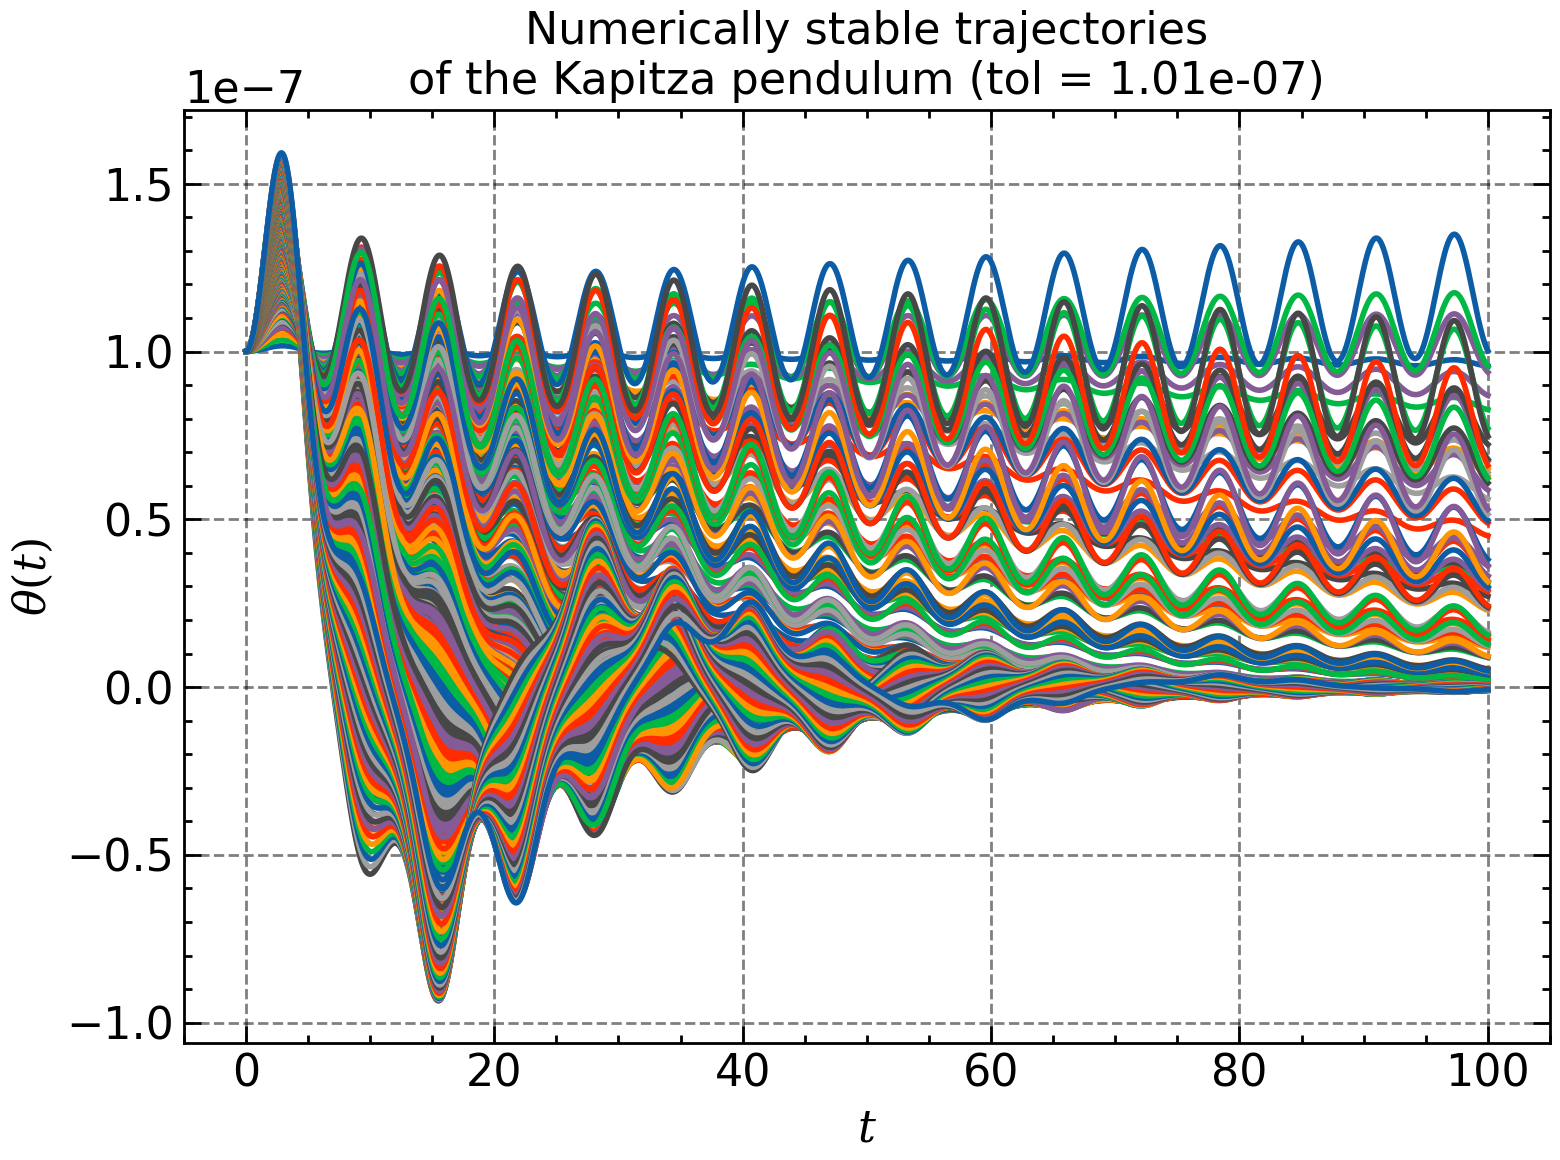
\includegraphics[width=0.75\linewidth]{Images/stable_trajs_1.01e-07.png}
%     \caption{Numerically stable trajectories.}
%     \label{fig:trajs}
% \end{figure}

The comparison demonstrates that the perturbative multiscale method, truncated to second order in $\epsilon$, correctly predicts the stability region, provided that the numerical simulations accurately replicate the physical behaviour of the system. It is also of interest to investigate the stability of the fixed point beyond the region of validity of the multiscale method. For instance, running simulations with the parameters shown in Table \ref{tab:pars2} reveals deviations from the multiscale prediction, as illustrated in Figure \ref{fig:phys_stab}.

\begin{table}[h]
    \centering
    \begin{tabular}{|c|c|} \hline 
        $\theta_0$ & $10^{-7}$ \\ \hline 
        $\omega_0$ & 0 \\ \hline 
         $\mu$& 1 \\ \hline
         $a$&  $0$ -- $1$\\ \hline
         $\sigma$&  $10^{-5}$ -- $0.1$\\ \hline
    \end{tabular}
    \caption{Parameter ranges.}
    \label{tab:pars2}
\end{table}

\begin{figure}[h]
    \centering
    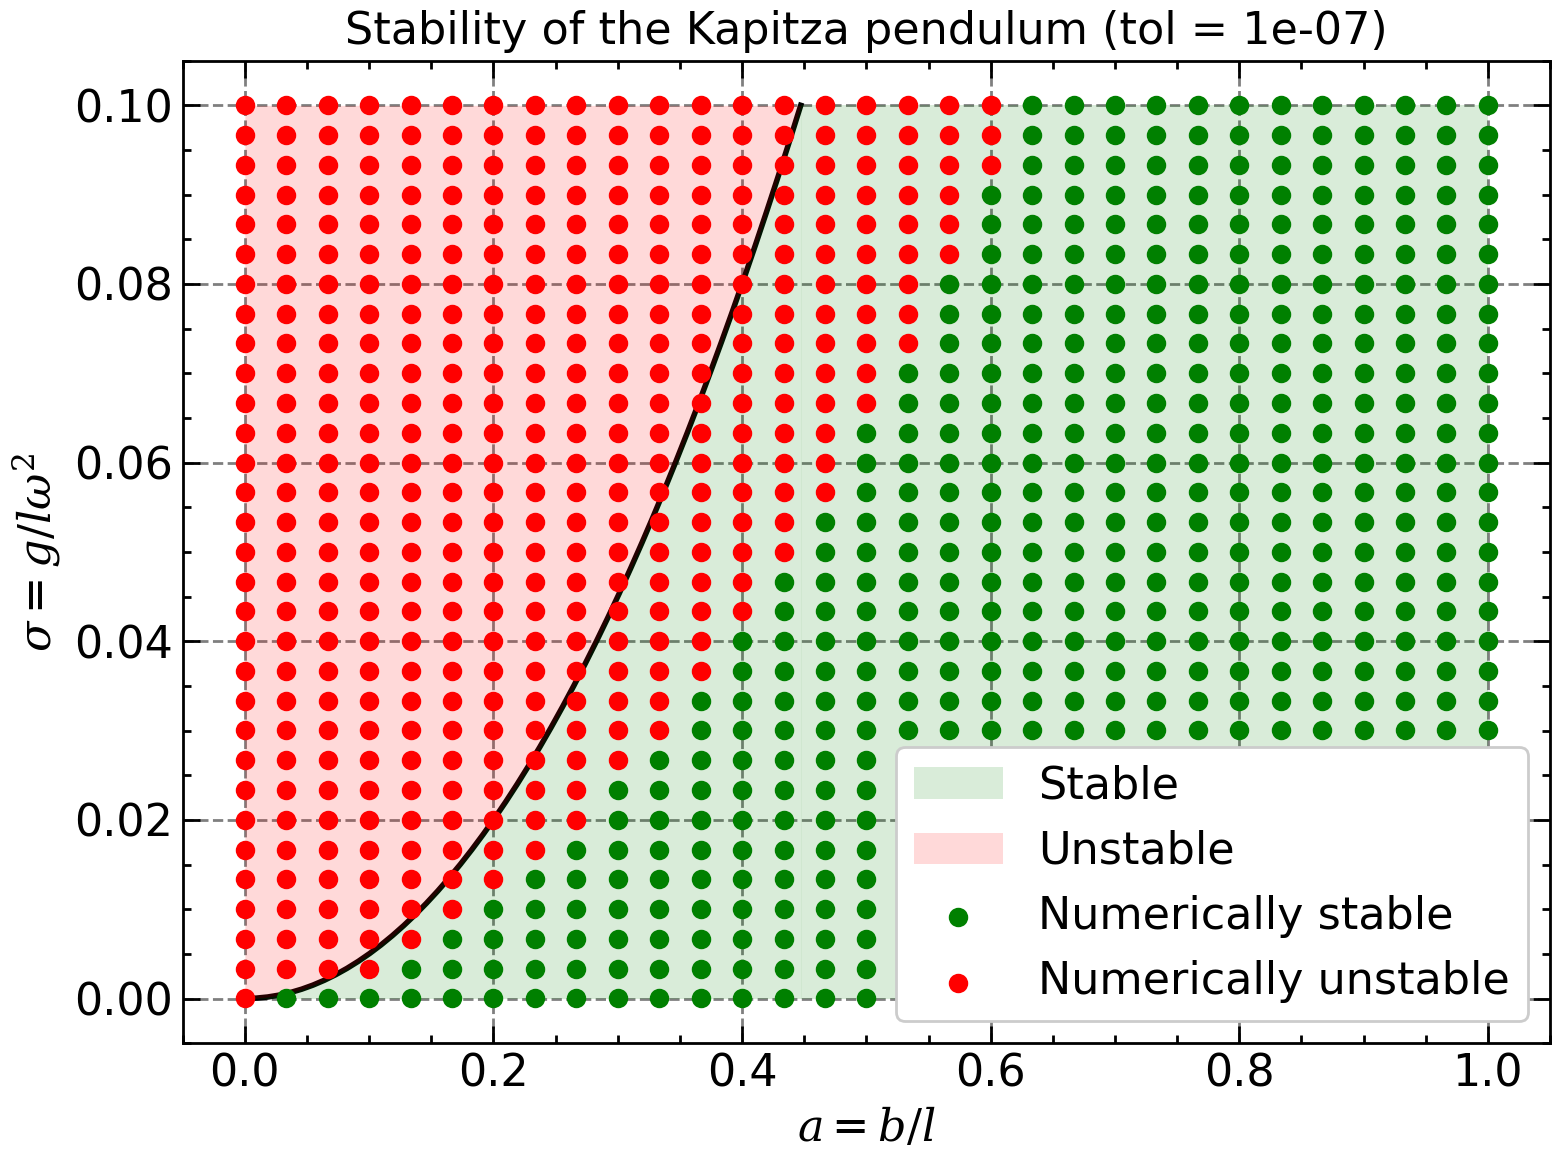
\includegraphics[width=0.75\linewidth]{Images/stability_1e-07.png}
    \caption{Stability of the upper fixed point beyond multiscale domain.}
    \label{fig:phys_stab}
\end{figure}

These results suggest that a higher-order multiscale approximation is required to accurately capture the physical behaviour of the Kapitza pendulum when the parameters extend beyond the validity region of the second-order perturbative solution. Alternatively, it may indicate that the system cannot be effectively studied using a perturbative method in this regime.
